\chapter{Methodology}\label{ch:methodology}
This chapter presents the methodological framework that underpins the research on multi-label classification for cybersecurity filtering and classification. This research aims to develop an effective system to analyze social media posts to raise awareness about cybersecurity threats. Social media platforms represent vast repositories of cybersecurity-related content. Still, there is a critical need to identify and focus on the relevant information in the overwhelming volume of posts. The classification system developed in this study addresses this need by effectively filtering and categorizing cybersecurity-related content.

A comprehensive understanding of the datasets is necessary before delving into system architecture design, as the characteristics of these datasets -- particularly their labeling structure and distribution -- directly inform the design choices in our classification approach. Therefore, the chapter begins with a detailed examination of the datasets employed in the study, outlining their sources, characteristics, and the preprocessing techniques used to ensure the quality and relevance of the data (Section \ref{sec:datasets-mtd}). This analysis of label distributions and dataset properties is crucial as it shapes the subsequent architectural decisions and model selection.

Following this foundational data analysis, the architectures developed to tackle the classification problem are presented. Section~\ref{sec:architecture} is devoted to the system architecture, which is further divided into two subsections: Section~\ref{subsec:two-step-system-mth} explains the Two-Step System -- where filtering of non-relevant content and subsequent categorization of relevant social media posts are handled in distinct stages -- and Section~\ref{subsec:one-step-system} describes the One-Step System, which integrates these tasks into a unified model to streamline processing and reduce error propagation. Finally, Section~\ref{sec:implementation-and-setup} outlines the implementation and experimental setup, covering the machine learning algorithms, embedding techniques, and evaluation metrics used to assess the performance of our proposed models. Together, these sections provide a comprehensive overview of the methods and procedures that form the foundation of this research.

\section{Datasets}\label{sec:datasets-mtd}
The need to ensure robustness and the ability to generalize in cybersecurity-related multi-label classification drove the selection of datasets for this study. Two complementary datasets -- NistPosts and CyberPosts -- were chosen based on their relevance to cybersecurity discussions on social media and their distinct characteristics regarding data collection methodology and content focus.

The works~\cite{cotov2023} and~\cite{behzadan2018} provided NistPosts and CyberPosts datasets respectively. The two sources describe different approaches to collecting and processing datasets of posts for cybersecurity analysis.

The NistPosts dataset is a collection of 24,474 posts available for the training and assessment steps. The dataset made available by the authors of~\cite{cotov2023} is made of social media posts extracted from Twitter using Twitter APIs. It combines the NIST CVE descriptions and the social media contents labeled as ``\texttt{informative}'' or ``\texttt{not informative}.'' These data were labeled with an active learning approach to prioritize the posts' evaluation based on their relevance probability. Those posts were joined with those belonging to a compact list of 36 Twitter users. To ensure the relevance of the obtained data, pertinent keywords were derived from the NIST website and a semi-manual selection process. The TWARC library was employed to enrich the dataset with additional data. Manual labeling proceeded to build up the datasets when data was collected. From a data quality perspective, duplicates and posts with very short text were eliminated.

The CyberPosts dataset is a collection of 21,368 posts curated directly from cybersecurity experts and made available by the authors of~\cite{behzadan2018}. The stream listener results were pre-filtered by keywords, including general words like ``\texttt{vulnerability}'' and ``\texttt{0day}'' and specific threat-related words like ``\texttt{DDoS}'' and ``\texttt{SQL injection}.'' The posts were pre-labeled in relevance and type to serve as suggestions in the annotation process, which four human cybersecurity experts performed concurrently on relevance and threat types. Then, IBM's Watson Natural Language Understanding service classified each post's textual content and made it available to experts to help annotate.

\begin{figure}
    \centering
    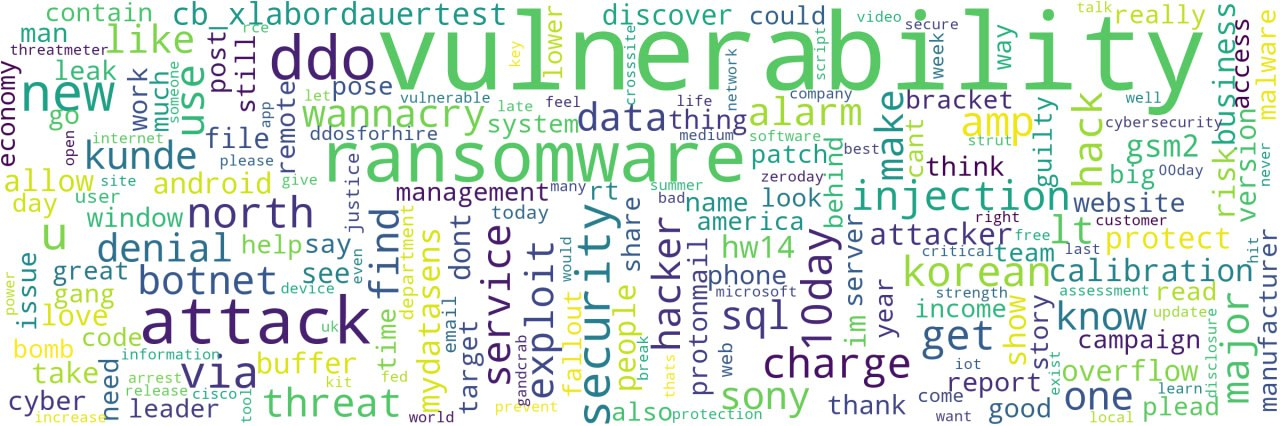
\includegraphics[width=1\linewidth]{Images/behzadan_wordcloud2}
    
\includegraphics[width=0.0625\linewidth]{Images/sep}
    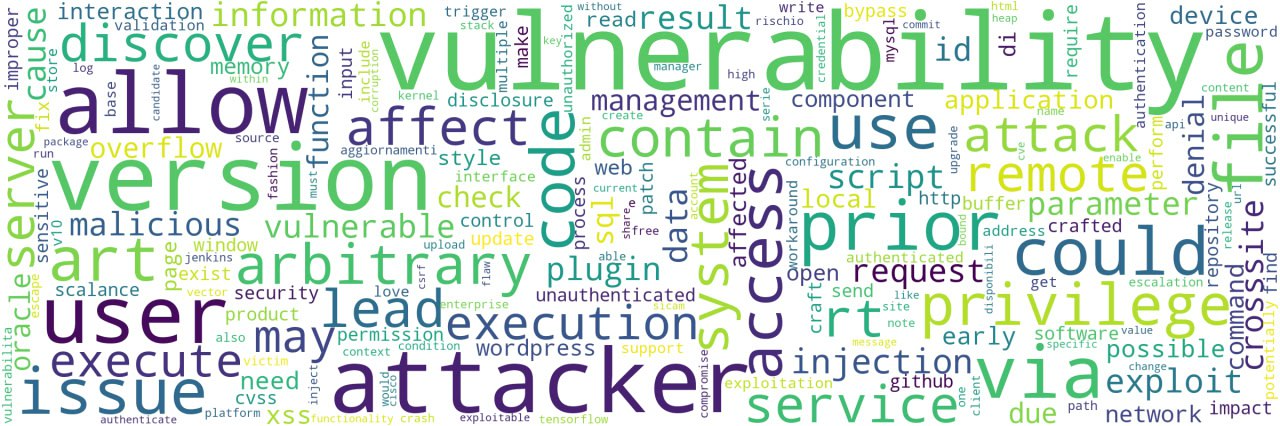
\includegraphics[width=1\linewidth]{Images/cotov_wordcloud}
    \caption{\textbf{Wordclouds} of the CyberPosts Dataset (top) and NistPosts Dataset (down).}
    \label{fig:wordclouds}
\end{figure}

By plotting the word clouds of the two datasets in Figure~\ref{fig:wordclouds}, the CyberPosts dataset shows more keywords related to cybersecurity topics than the NistPosts dataset. To quantify these differences, word distributions were plotted. The vocabulary overlap analysis showed that CyberPosts contained frequent words directly related to cybersecurity (e.g., \texttt{vulnerability}, \texttt{ransomware}, \texttt{attack}, \texttt{ddos}, \texttt{exploit}, \texttt{security}, \texttt{injection}, \texttt{sql}) for both the relevant and irrelevant posts. In contrast, NistPosts had way fewer cybersecurity-related words in the irrelevant posts, with the frequent words being more generic (e.g., \texttt{art}, \texttt{style}, \texttt{love}, \texttt{fashion}, \texttt{good}, \texttt{like}).

\begin{figure}
    \centering
    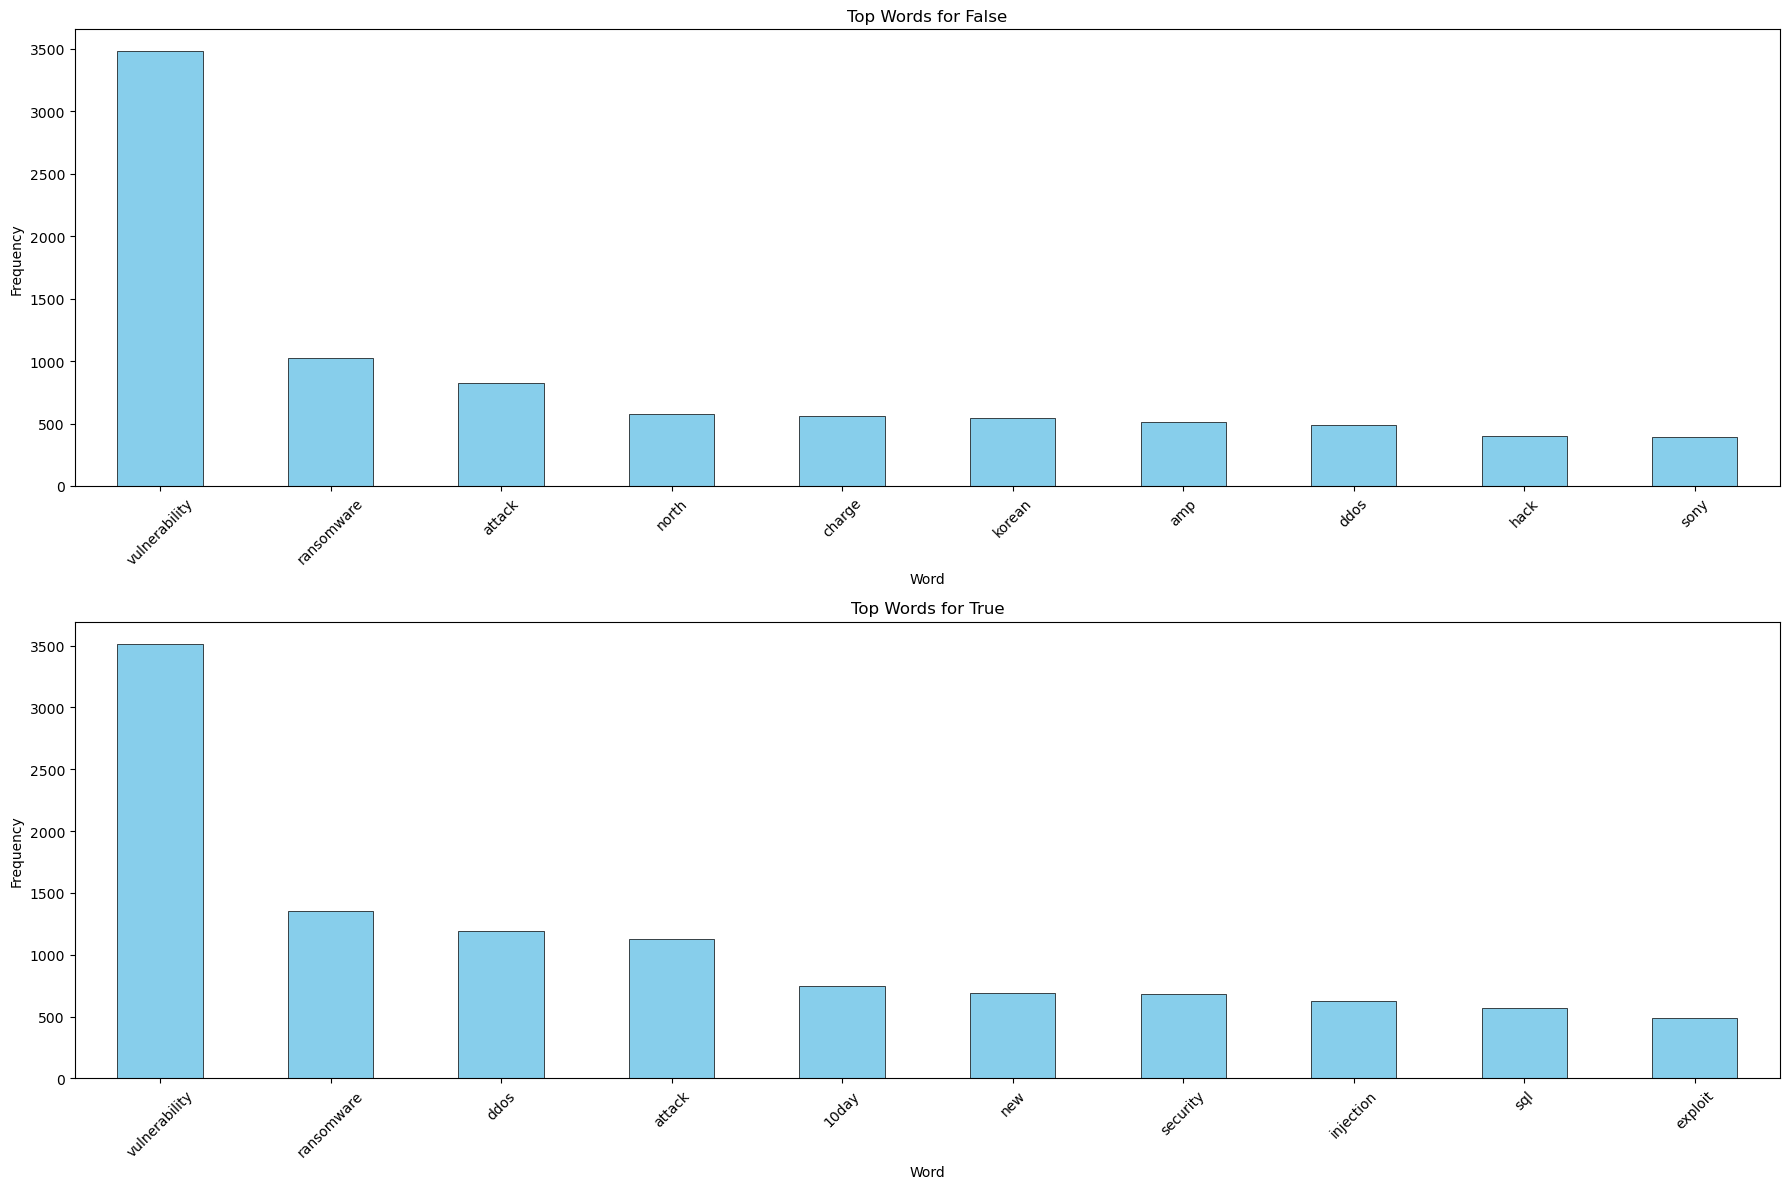
\includegraphics[width=1\textwidth]{Images/behzadan_words_distribution}
    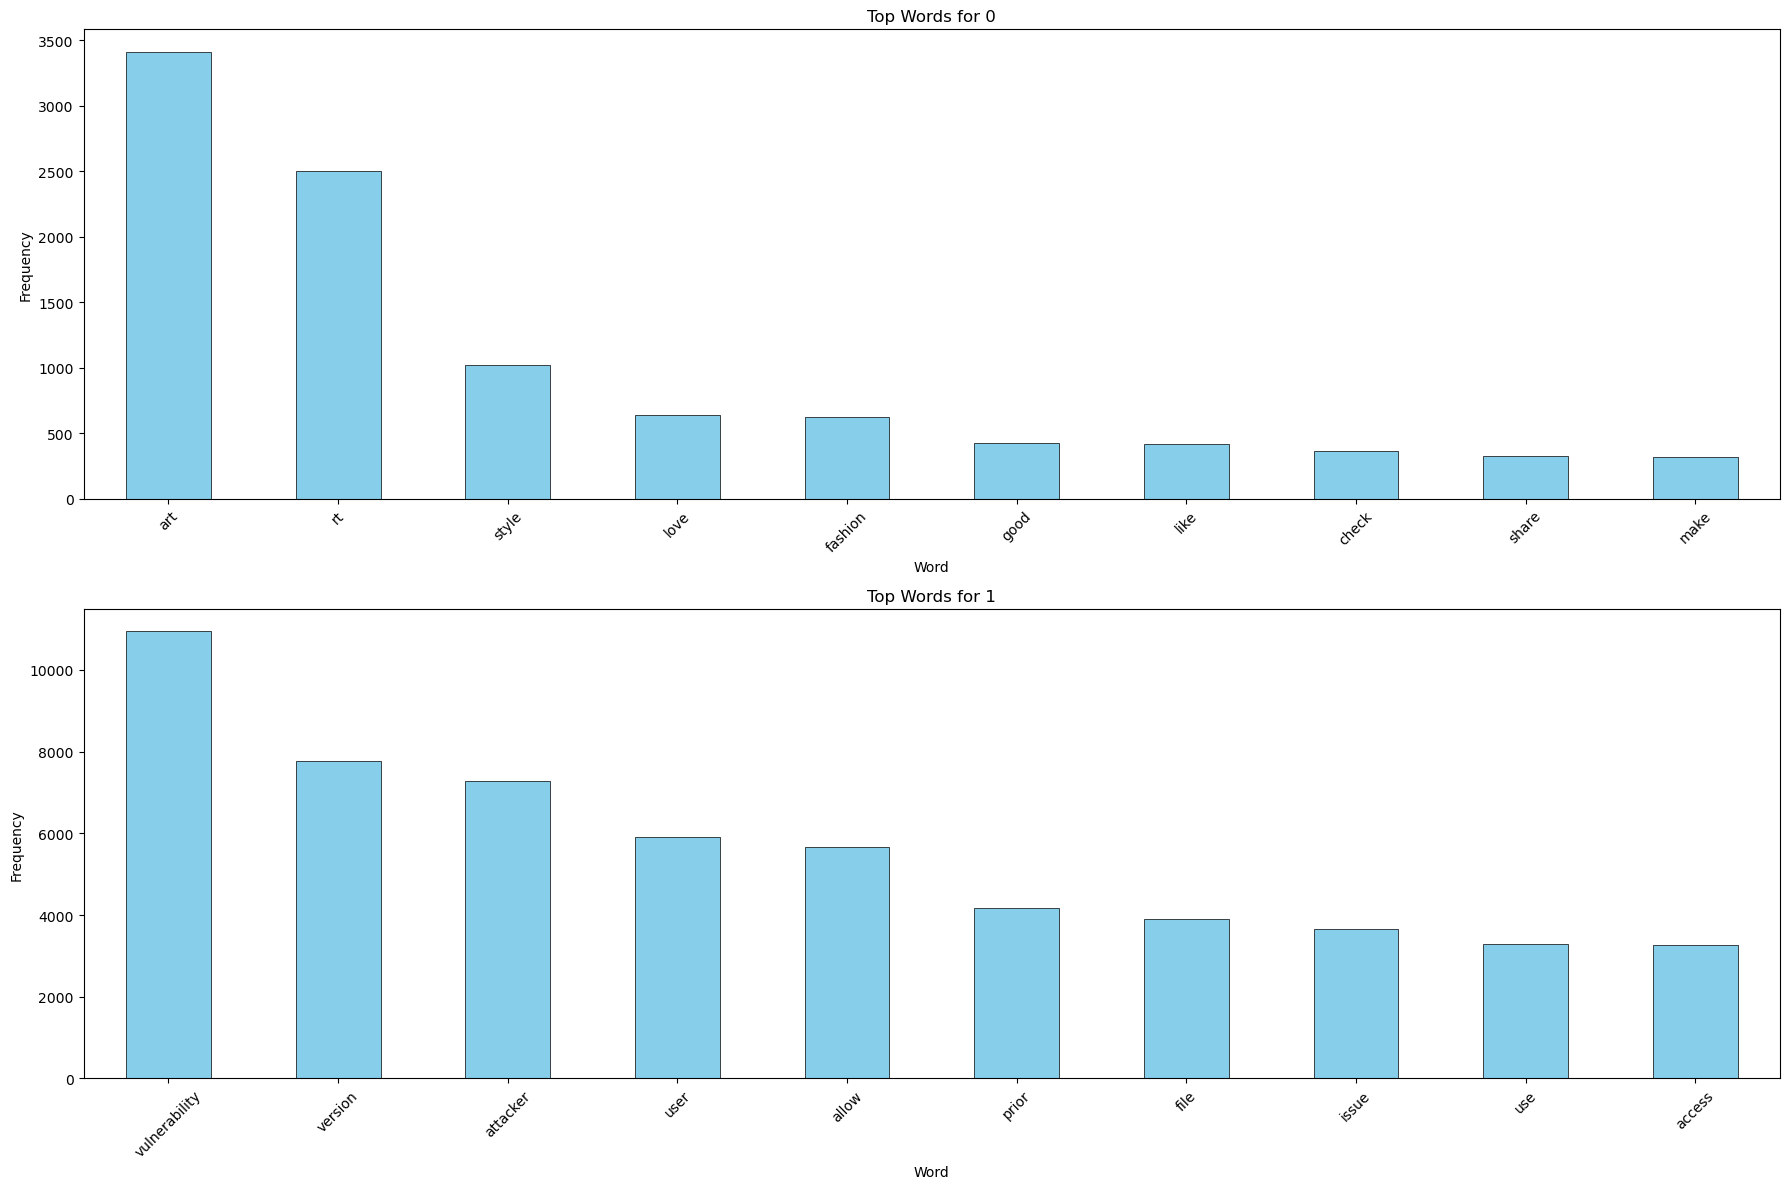
\includegraphics[width=1\textwidth]{Images/cotov_words_distribution}
    \caption{\textbf{Words Distribution} in CyberPosts Dataset (top) and NistPosts Dataset (down).}
    \label{fig:words-distribution}
\end{figure}

Figure~\ref{fig:words-distribution} shows that in CyberPosts, both relevance labels (0 and 1) contained a significant proportion of cybersecurity-related terms, making it a more suitable dataset for training a cybersecurity filter. In contrast, NistPosts showed a higher imbalance where label 0 (non-relevant) consisted of primarily non-cybersecurity terms, and label 1 (relevant) contained cybersecurity-related terms.

Even if the wordclouds (Figure~\ref{fig:wordclouds}) showed that some common keywords were evenly distributed, the word distribution analysis showed an imbalanced distribution across the two labels. For this reason, the classifiers were trained using the CyberPosts dataset to ensure they would be more robust in learning the post's underlying patterns. Ultimately, the NistPosts dataset was used as a second evaluation set to validate the models.

The CyberPosts dataset has different columns that can interest the implementation of a classifier; however, for obvious reasons, this study uses the ``\texttt{text}'' column, the ``\texttt{relevant}'' column for training and testing the binary classifier filter, and the ``\texttt{watson}'' column for training and testing the multi-label classifier model for assigning categories to posts. The ``\texttt{annotation}'' field is another interesting column since it contains the labeling of cybersecurity experts. Still, it was not used since its values were not considered essential for linking the posts to the nodes of companies' system graphs.

\begin{figure}
    \centering
    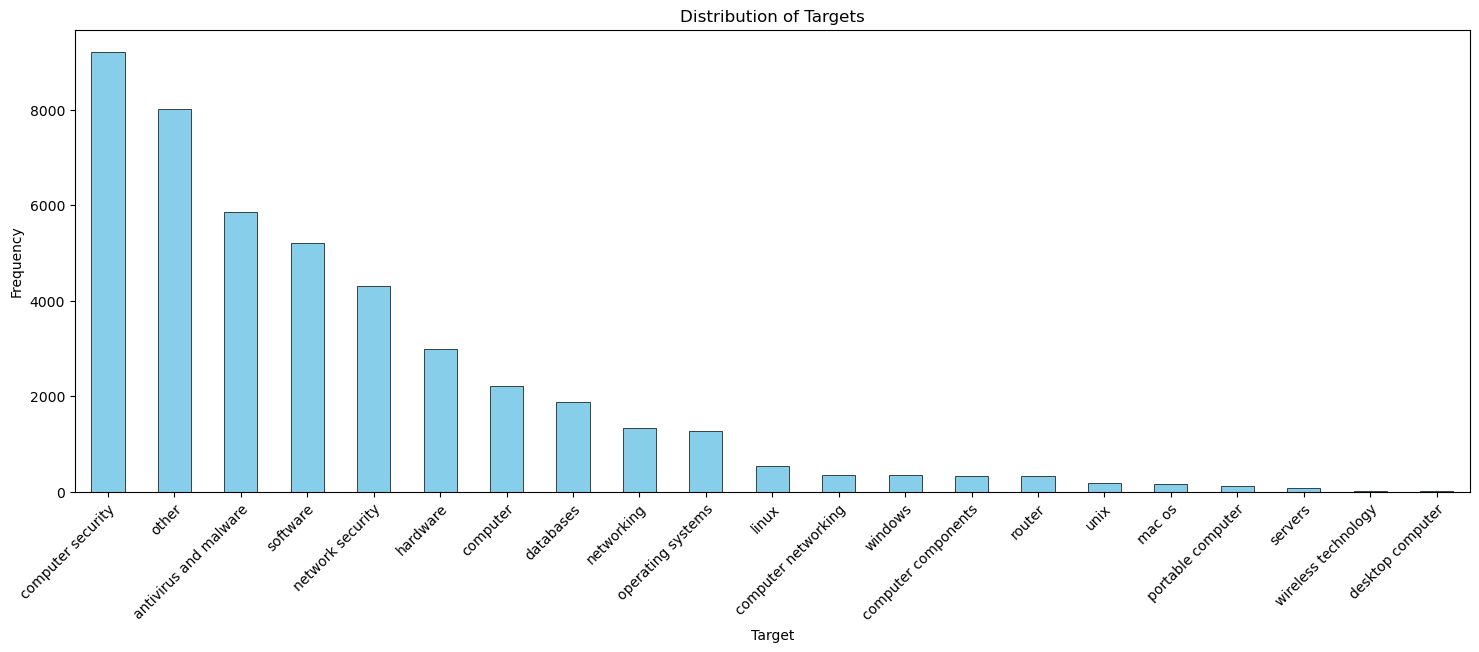
\includegraphics[width=1\linewidth]{Images/behzadan_target_distribution}
    \caption{\textbf{Distribution of Categories in CyberPosts Dataset}.}
    \label{fig:cyber-posts-target-distribution}
\end{figure}

A weak point of the CyberPosts dataset is its strongly imbalanced dataset for the MLC task (Figure~\ref{fig:cyber-posts-target-distribution}). The most common label among the posts is ``\texttt{Computer Security},'' with 9,216 samples associated. Then, at the second position, there is the ``\texttt{Other}'' label with 8,013 samples, which already highlights the imbalance. Still, in the third position, the label ``\texttt{Antivirus and Malware}'' with 5,854 samples, followed by the label ``\texttt{Software}'' with 5,214 samples, half of the most common label.


\section{Architecture}\label{sec:architecture}
\begin{figure}
    \centering
    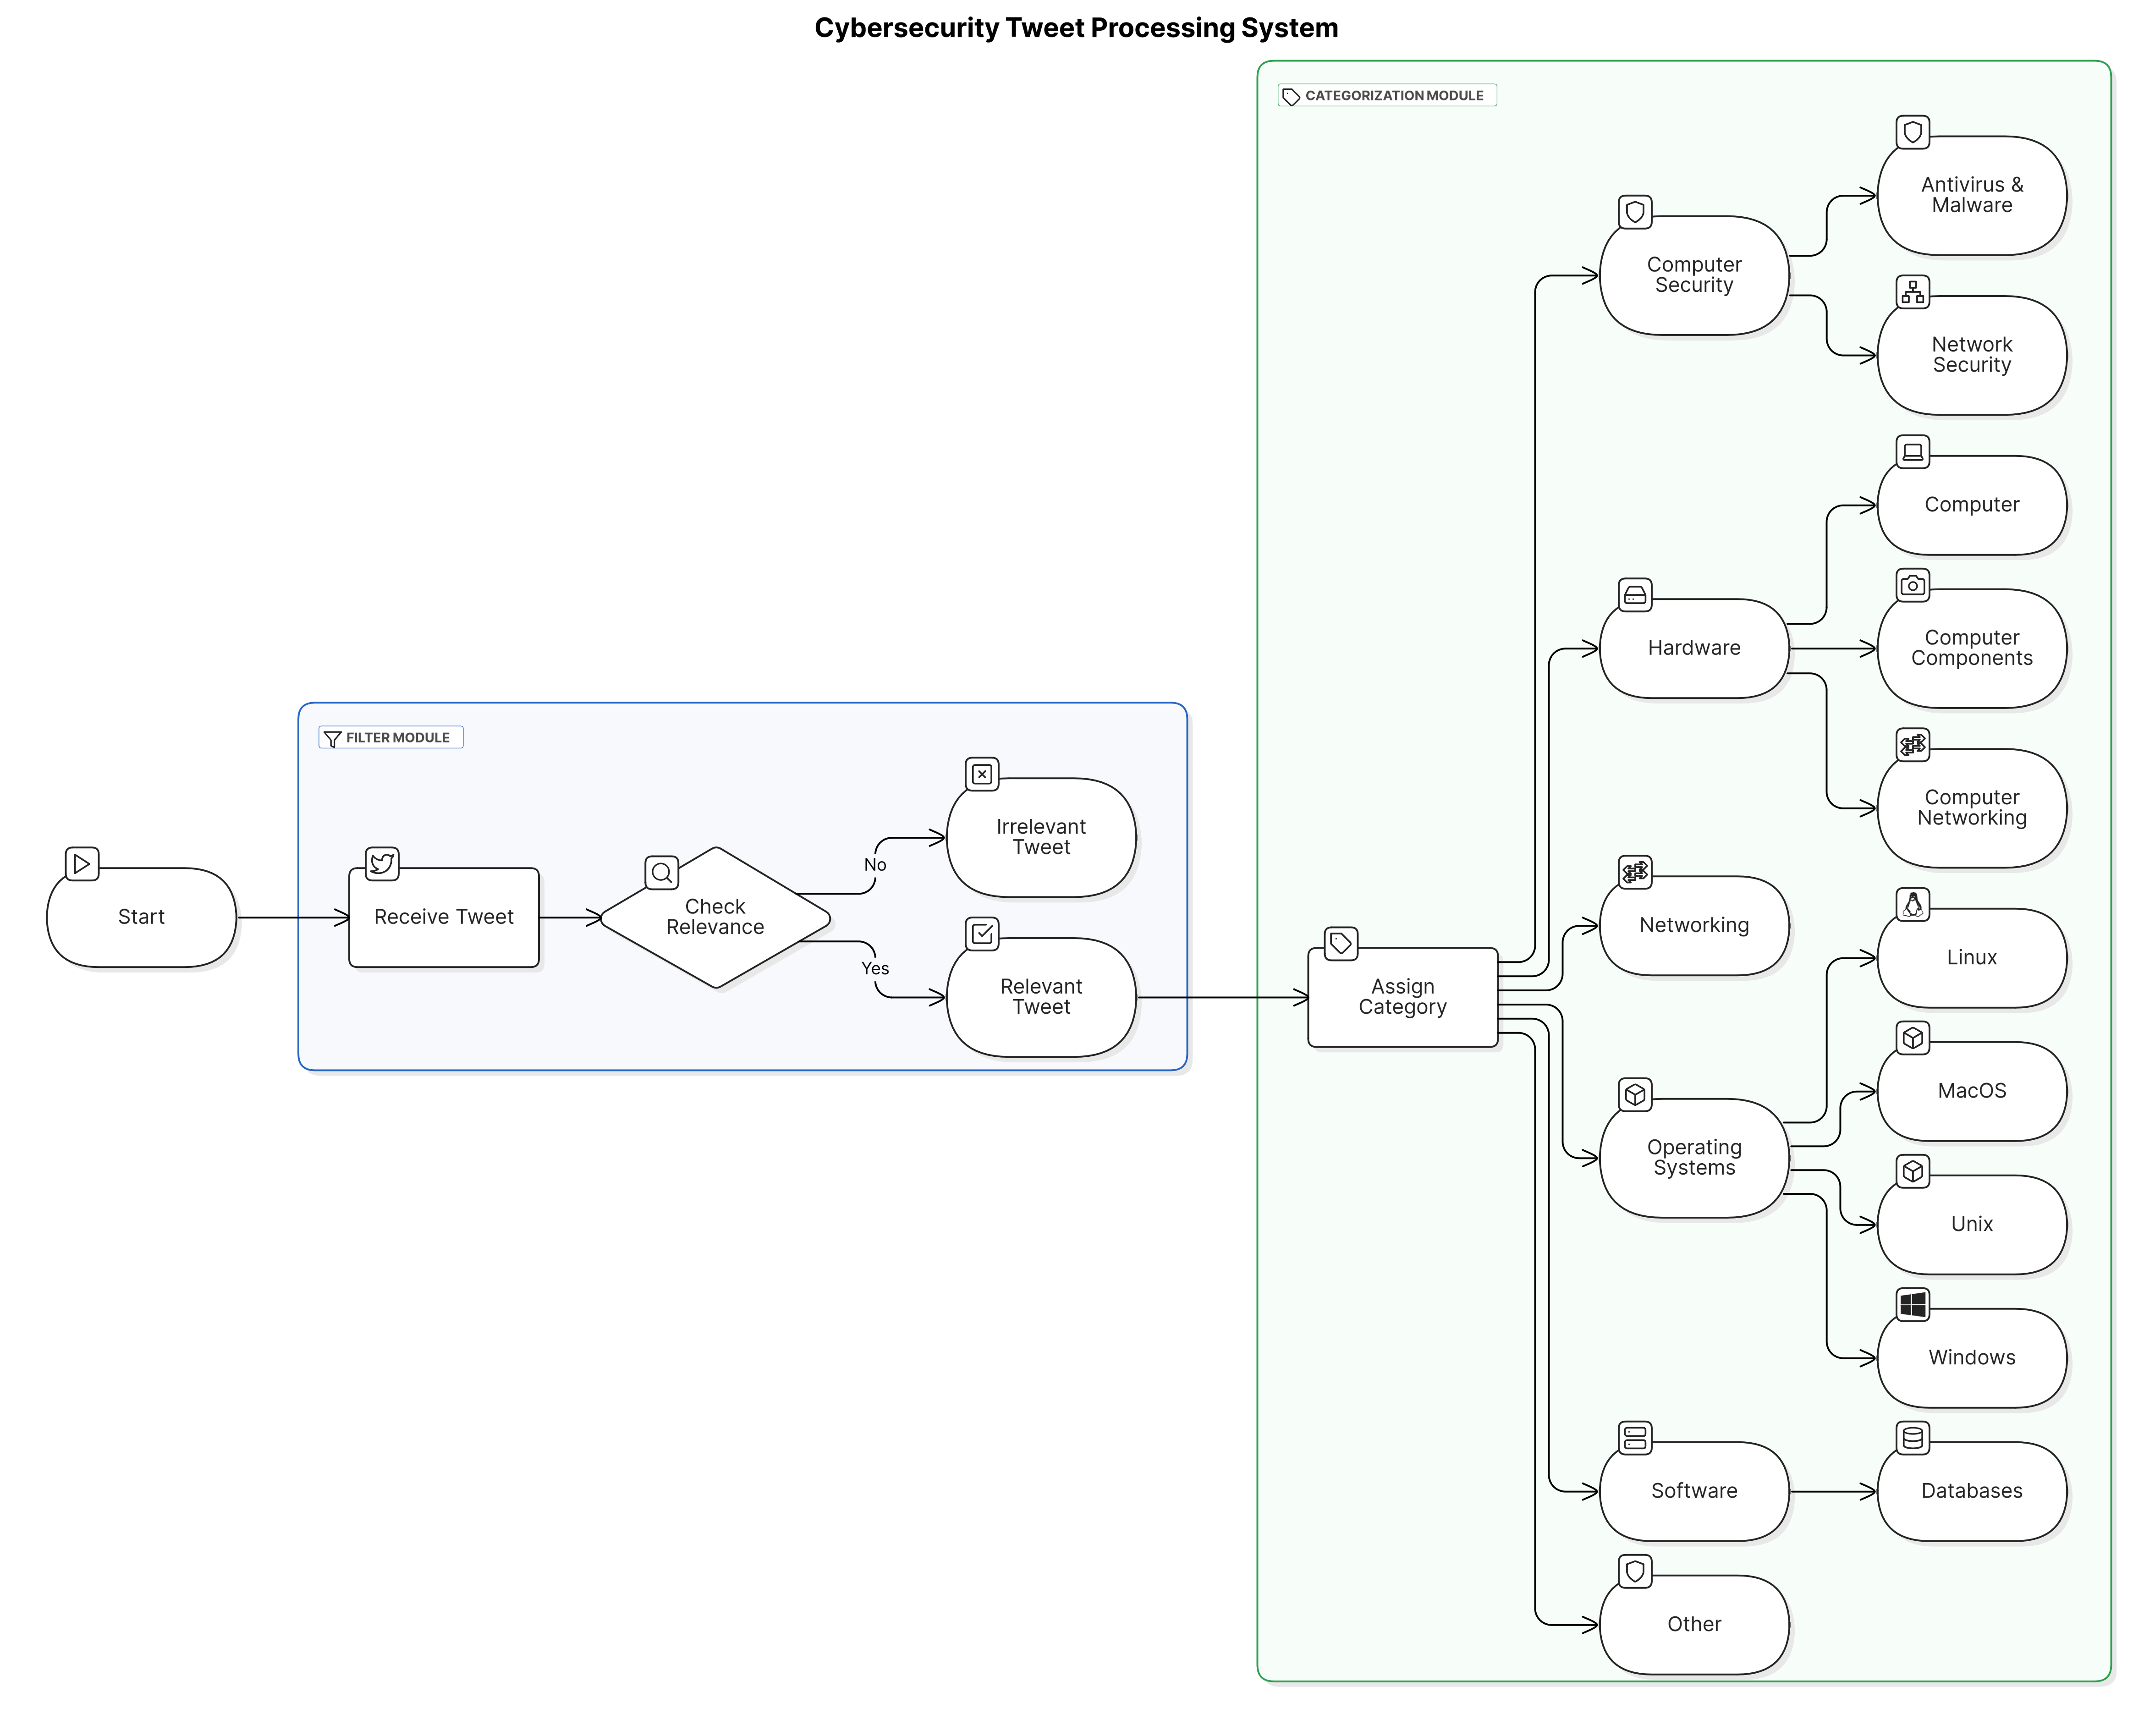
\includegraphics[width=\linewidth]{Images/system-schema-horizontal-new}
    \caption{\textbf{The Two-Step System's Architecture}.}
    \label{fig:two-step-system}
\end{figure}

The proposed system is a hierarchical multi-label classification approach. It operates in two structured levels: an initial classification into broad categories and a secondary classification into subcategories when applicable. This architecture ensures an interpretable classification process and enhances the precision of the multi-label classification predictions.

Once the categories are fixed, a deterministic mapping is applied to the list to map each category to a node type in system graphs.



\subsection{The Two-Step System}\label{subsec:two-step-system-mth}
In the Two-Step System, there are two modules: the \textit{Filter module} filters out all the posts irrelevant to cybersecurity topics, and the \textit{Categorization module} assigns hierarchical categories to each post considered relevant for end users.

Figure~\ref{fig:two-step-system} visually presents the system flow. Incoming posts are preprocessed by removing URLs, emails, mentions, and hashtags. Then, the embeddings are computed for each post, and the binary classification models predict its relevance. Then, the second module assigns categories to the posts predicted as relevant. The Categorization module is formed by two layers of models that classify posts into high-level categories (\texttt{Computer Security}, \texttt{Hardware}, \texttt{Networking}, \texttt{Operating Systems}, \texttt{Other}, and \texttt{Software}), and then classify posts into subcategories within the high-level categories, if applicable, as follows:

\begin{itemize}
    \item \texttt{Computer Security} $\rightarrow$ \texttt{Antivirus and Malware}, \texttt{Network Security}
    \item \texttt{Hardware} $\rightarrow$ \texttt{Computer}, \texttt{Computer Components}, \texttt{Computer Networking}
    \item \texttt{Operating Systems} $\rightarrow$ \texttt{Linux}, \texttt{MacOS}, \texttt{Unix}, \texttt{Windows}
    \item \texttt{Software} $\rightarrow$ \texttt{Databases}
\end{itemize}

For example, if a post is classified under \texttt{Hardware}, it is re-evaluated for the specific subcategories like \texttt{Computer Components}. If no subcategory is applicable, the classification remains in the high-level category.

\subsection{The One-Step System}\label{subsec:one-step-system}
The One-Step System integrates Filtering and Categorization modules to increase the filter's performance and avoid error propagation into the category classifier. In this case, the CyberPosts target for the MLC task was manipulated by forcing the irrelevant posts to have category ``\texttt{Other}'', so in the training phase, the models will learn to predict a category whenever the post is relevant, and ``\texttt{Other}'' otherwise. So, the system consists of five primary models trained to classify posts into high-level categories and subcategories, like the Two-Step System.

For example, given a list of posts, each post is processed by the embeddings and encoders. Then the models predict the categories among the high-level categories -- \texttt{Computer Security}, \texttt{Hardware}, \texttt{Networking}, \texttt{Operating Systems}, \texttt{Other}, and \texttt{Software}. As already said, the significant advantage of the One-Step System is that the filter and categorization modules are trained together because they are part of the same model. Consequently, when a post is recognized as irrelevant by the first layer category classifier, the model will assign only the category ``\texttt{Other}'' to the post, and the second layer category classifier will not be involved in the prediction. For all the relevant posts, the system will predict not only the high-level category but also the subcategories, and most importantly, it will not assign category ``\texttt{Other}'' to the relevant posts since it is forced to predict a category whenever the post is relevant.

\section{Implementation and Setup}\label{sec:implementation-and-setup}
In this section, the architecture implementation described in Section~\ref{sec:architecture} is presented, detailing the datasets used, the data preprocessing steps, the embedding models, the classification models, and the evaluation metrics employed to assess the models' performance.

\subsection{Datasets}\label{subsec:datasets-imp-stp}
\begin{figure}
    \centering
    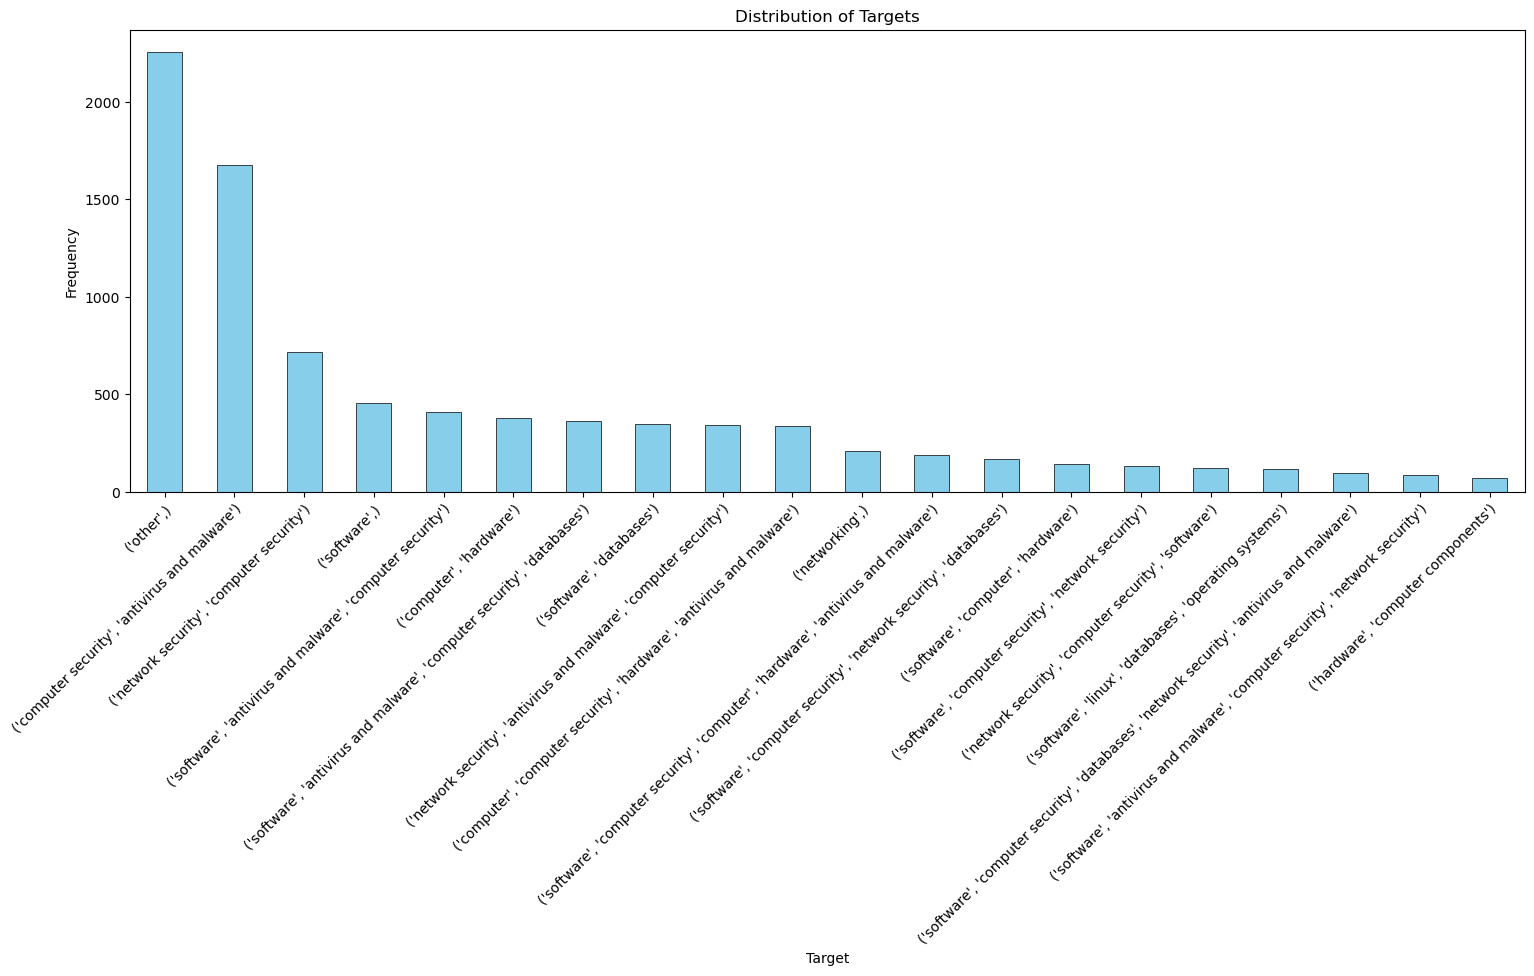
\includegraphics[width=1\linewidth]{Images/behzadan_target_set_distribution}
    \caption{\textbf{Distribution of Label-Sets in CyberPosts Dataset}.}
    \label{fig:cyber-posts-target-set-distribution}
\end{figure}

Since the CyberPosts dataset is strongly imbalanced, as highlighted in Figure~\ref{fig:cyber-posts-target-distribution}, the models have many difficulties generalizing the information to new unseen data. Another plot that helps understand the challenges in training for methods such as the Label Powerset algorithm is the Figure~\ref{fig:cyber-posts-target-set-distribution}, where the label-set ``\texttt{(Other)}'' is the most common with 2,255 samples, followed by ``\texttt{(Computer Security, Antivirus and Malware)}'' with 1,674 samples and ``\texttt{(Network Security, Computer Security)}'' with 719 samples.

Because of the distributions in Figure~\ref{fig:cyber-posts-target-distribution} and Figure~\ref{fig:cyber-posts-target-set-distribution}, it was expected to have higher performances with methods that did not consider the label dependencies, like the Binary Relevance algorithm, and lower performances with methods that considered the label dependencies, like the Label Powerset algorithm.

\subsection{Data Preprocessing}\label{subsec:data-preprocessing}
With the choice of not enhancing the posts with external information but the embeddings and encoders, there were defined models that only received text embeddings, so the embedding models had prior roles in the success of the training steps.

Before feeding the texts to the embeddings, a data cleaning process was performed to remove all the noises from the posts. In particular, the emails, URLs, mentions, and hashtags were removed since they were not considered informative for the posts.

For the training of the binary classification models, the posts were split into training and testing sets with an 80{\%} and 20{\%} ratio, respectively. The split was performed with the \texttt{train\_test\_split} function from the \texttt{scikit-learn} library by stratifying the data to ensure that the distribution of the classes was the same in both the training and testing sets.

The datasets for training and evaluating the multi-label classification models depended on the architecture used. For the Two-Step System, the data were filtered to retain only the posts relevant to cybersecurity topics, independently of the predictions of the filter modules. For the One-Step System, the data were manipulated to force the irrelevant posts to have the category ``\texttt{Other}'', so all the posts were used to train the models.

For the training of the two multi-label classification architectures, the posts were split into training and testing sets with an 80{\%} and 20{\%} ratio, respectively. In this case, the label sets were stratified to ensure that the distribution of the label sets was the same in both the training and testing sets. However, the label sets were poorly distributed in the dataset, so the split required discarding the samples associated with rare label sets. In particular, only the posts with label sets with at least 20 samples were considered for the training and testing split.


\subsection{Embeddings Models}\label{subsec:embeddings-models}
Across the experiments, the embeddings and encoders presented in Section~\ref{subsubsec:the-embeddings} were used: the embeddings to convert the posts into numerical vectors and the encoders to compute the post embeddings.

The chosen GloVe{\footnote{\href{https://nlp.stanford.edu/projects/glove/}{GloVe: Global Vectors for Word Representation}}} embeddings contained six billion tokens. Whenever words were not in GloVe's vocabulary, they were discarded as they were translated into zero vectors. It was the same for all the GloVe versions, namely the 50, 100, 200, and 300-dimensions. Ideally, the 50-dimension embeddings only captured the general text semantics. Still, they should not be informative enough for tasks such as assigning categories potentially correlated to each other in computer science. For this reason, it was expected to notice higher performances with the 300-dimensional embeddings among all the four static embeddings.

Since static embeddings are not generally used in state-of-the-art natural language processing applications, the encoders were applied to compute the post embeddings.

The SBERT{\footnote{\href{https://huggingface.co/sentence-transformers/all-mpnet-base-v2}{sentence-transformers/all-mpnet-base-v2}}} and DistilRoBERTa{\footnote{\href{https://huggingface.co/sentence-transformers/all-distilroberta-v1}{sentence-transformers/all-distilroberta-v1}}} were the first to be tested. Finally, the ATT{\&}CK-BERT{\footnote{\href{https://huggingface.co/basel/ATTACK-BERT}{basel/ATTACK-BERT}}} encoder was employed to increase accuracies and robustness. All of them were computed with the \texttt{sentence-transformers} library in Python.

\subsection{Classification Models}\label{subsec:classification-models}
For the training of the \textbf{Filter module} of the Two-Step System, the binary classification models were used to predict the relevance of the posts.

There were constructed 28 models by combining the four embeddings presented in Section~\ref{subsubsec:the-embeddings} (GloVe 6B 50D, GloVe 6B 100D, GloVe 6B 200D, and GloVe 6B 300D), and three encoders presented in Section~\ref{subsubsec:the-encoders} (DistilRoBERTa, SBERT, and ATT{\&}CK-BERT) with the four base classifiers presented in Section~\ref{subsec:binary-classification} (Logistic Regression, Naïve Bayes, Random Forest, and XGBoost).

Each model was implemented as a simple \texttt{scikit-learn} pipeline with a standard scaler as the first layer and the classifier as the second layer. The standard scaler only normalizes the data by centering the mean of the embeddings to 0 and their variance to a unit standard deviation. This normalization technique helps the algorithms in learning more efficiently without the need for scaling factors.

The best model for the Filter module was selected based on the highest mean cross-validation accuracy, with a cross-validation of 5 folds. Once the model was identified, it was hyperparameter-tuned with a Bayesian optimization technique using the \texttt{hyperopt} library in Python.

In the \textbf{Categorization module} and for both the architectures, the algorithms used for the binary classification task could not solve the problem, as for Logistic Regression, or were inefficient, as for Naïve Bayes, so state-of-the-art methods for solving multi-label classification tasks were used.

The multi-label classifiers for assigning categories to relevant posts are built manually by following the pseudocode presented in \cite{zhang2014}. In this case, the methods used for facing the problem were the same as explained in Section~\ref{subsec:multilabel-classification} (BR, CLR, CC, LP, PSt, MBR, RAkEL, and HOMER), combined with each base classifier presented in Section~\ref{subsec:binary-classification}, for all the embeddings and encoders: there were trained more than 200 models.

The best model for the Categorization module was selected based on the highest macro F1 score.

\subsection{Evaluation Metrics}\label{subsec:evaluation-metrics}
Different metrics were used to assess all the models and extract only those relevant to solving the two tasks (filter and categorization). The metrics include:
\begin{itemize}
    \item \textbf{Accuracy}. It is the number of correct classification predictions divided by the total number of predictions.
    \item \textbf{Precision}. It is the proportion of all the model's positive classifications that are actually positive.
    \item \textbf{Recall} (or True Positive Rate, TPR). It is the proportion of all actual positives classified correctly as positives.
    \item \textbf{F1 score}. It is the harmonic mean of precision and recall. This metric balances the importance of precision and recall and is preferable to accuracy for class-imbalanced datasets. More broadly, when precision and recall are close in value, F1 will be close to their value. When precision and recall are far apart, F1 will be similar to whichever metric is worse.
    \item \textbf{AUC} (Area Under the ROC Curve). It represents the probability that the model will rank the positive higher than the negative if given a randomly chosen positive and negative example.
    \item \textbf{Hamming loss}. It is a metric that computes the fraction of wrong labels to the total number of labels. It is used in multi-label classification and penalizes only the individual labels. A lower Hamming loss indicates better performance.
    \item \textbf{Macro Averaging}. This approach independently computes metrics like precision, recall, and F1-score for each label and then averages them. It treats all labels equally, making it suitable when they are equally important, but it may not accurately reflect performance if label frequencies vary significantly.
    \item \textbf{Micro Averaging}. This approach globally computes metrics by aggregating contributions from all labels. This method is more sensitive to labels with higher frequencies and is beneficial when labels have varying importance or imbalance. Notably, in multi-class evaluation, micro F1 is equivalent to accuracy. 
    \item \textbf{Sample-based Averaging}. This approach computes metrics for each instance individually and averages these scores across all instances. It provides a balanced view of precision and recall at the instance level, offering a nuanced assessment of model performance.
    \item \textbf{Weighted Averaging}. This approach computes metrics that account for the imbalance in class distribution by considering each class's support (i.e., the number of true instances). This approach ensures that the performance metrics -- such as precision, recall, and F1-score -- reflect the contribution of each class proportionally to its occurrence in the dataset.
\end{itemize}

For the Two-Step System, the metrics were computed for the filter and Categorization modules to evaluate the system's performance comprehensively. For the One-Step System, the metrics were calculated for the whole system, as the Filter and Categorization modules were integrated into a single model.

In particular, for the aggregated performances of the Two-Step System, the metrics of the Categorization module were evaluated only on the relevant posts, so the irrelevant posts were not considered in the evaluation.